\documentclass{article}%standalone can be used
\usepackage{tikz}
\usetikzlibrary{shapes.geometric, calc}

\begin{document}
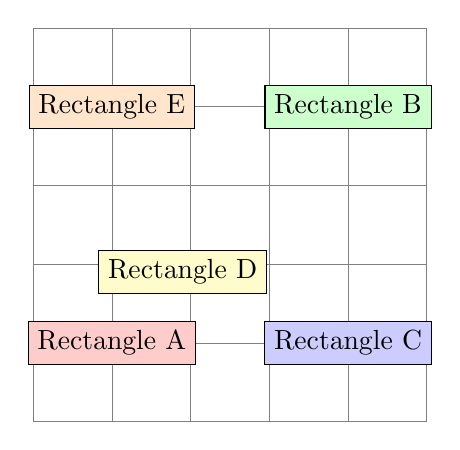
\begin{tikzpicture}
  \draw[style=help lines] (0, 0) grid (5, 5);
  \node (a) [rectangle, draw, fill=red!20]   at (1, 1) {Rectangle A};
  \node (b) [rectangle, draw, fill=green!20] at (4, 4) {Rectangle B};
  \node (c) [rectangle, draw, fill=blue!20]  at (b|-a) {Rectangle C};
  \node (d) [rectangle, draw, fill=yellow!20] at ($(a)!0.3!(b)$) {Rectangle D};
  \node (e) [rectangle, draw, fill=orange!20]  at (a|-b) {Rectangle E};
\end{tikzpicture}
\end{document}
